\documentclass[titlepage]{report}
\usepackage[backend=biber,style=numeric]{biblatex}
\addbibresource{literature.bib}
\usepackage{caption}
\usepackage{subcaption}
\usepackage{graphicx}
\usepackage[utf8]{inputenc}
\usepackage[T1]{fontenc}
\usepackage{url}
\usepackage{hyphenat}
\usepackage{glossaries}
\usepackage{array}
\usepackage{calc}
\usepackage{booktabs}
\usepackage{hyperref}
\usepackage{listings}
% \usepackage{xcolor} https://tex.stackexchange.com/q/466147
\usepackage{bytefield}
\usepackage{float}
\usepackage{eurosym}
\usepackage{tabu}
\usepackage{caption}
\usepackage{csquotes}
\lstset{%
    frame=tb,
    tabsize=4,
    numbers=left,
    breaklines=true,
}
\setcounter{biburllcpenalty}{9001}
\makeglossaries{}
\newglossaryentry{ima}
{%
    name={IMA},
    description={Computer network airborne system},
    first={Integrated Modular Avionics (IMA)},
    long={Integrated Modular Avionics}
}
\newglossaryentry{dima}
{%
    name={DIMA},
    description={Distributed computer network airborne system},
    first={Distributed Integrated Modular Avionics (DIMA)},
    long={Distributed Integrated Modular Avionics}
}
\newglossaryentry{apex}
{%
    name={APEX},
    description={APplication/EXecutive Interface},
    first={APplication/EXecutive Interface (APEX)},
    long={APplication/Executive Interface}
}
\newglossaryentry{coex}
{%
    name={COEX},
    description={COre/EXecutive Interface},
    first={COre/EXecutive Interface (APEX)},
    long={COre/Executive Interface}
}
\newglossaryentry{arinc}
{%
    name={ARINC},
    description={Aeronautical Radio Incorporated},
    first={Aeronautical Radio Incorporated (ARINC)},
    long={Aeronautical Radio Incorporated}
}
\newglossaryentry{aeec}
{%
    name={AEEC},
    description={Airlines Electronic Engineering Committee},
    first={Airlines Electronic Engineering Committee (AEEC)},
    long={Airlines Electronic Engineering Committee}
}
\newglossaryentry{lru}
{%
    name={LRU},
    description={Line-Replaceable Unit},
    first={Line-Replaceable Unit (LRU)},
    long={Line-Replaceable Unit},
    plural={LRUs},
    firstplural={Line-Replacable Units (LRUs)}
}
\newglossaryentry{lrm}
{%
    name={LRM},
    description={Line-Replaceable Module},
    first={Line-Replaceable Module (LRM)},
    long={Line-Replaceable Module},
    plural={LRMs},
    firstplural={Line-Replacable Modules (LRMs)}
}
\newglossaryentry{arinc429}
{%
    name={ARINC 429},
    description={ARINC standard for a global data bus in aviation},
    first={ARINC 429 standard},
    long={ARINC 429 standard}
}
\newglossaryentry{arinc629}
{%
    name={ARINC 629},
    description={ARINC standard for a global computer bus in aviation},
    first={ARINC 629 standard},
    long={ARINC 629 standard}
}
\newglossaryentry{arinc650}
{%
    name={ARINC 650},
    description={ARINC standard for IMA packaging and interfaces},
    first={ARINC 650 standard},
    long={ARINC 650 standard}
}
\newglossaryentry{arinc651}
{%
    name={ARINC 651},
    description={ARINC report that provides guidelines for a maintenance strategy for IMA-equipped airplanes},
    first={ARINC 651 report},
    long={ARINC 651 report}
}
\newglossaryentry{arinc653}
{%
    name={ARINC 653},
    description={ARINC standard for space and time partitioning},
    first={ARINC 653 standard},
    long={ARINC 653 standard}
}
\newglossaryentry{arinc659}
{%
    name={ARINC 659},
    description={ARINC standard for a backplane data bus},
    first={ARINC 659 standard},
    long={ARINC 659 standard}
}
\newglossaryentry{RTCA}
{%
    name={RTCA},
    description={Radio Technical Commission for Aeronautics (RTCA)},
    first={Radio Technical Commission for Aeronautics (RTCA)},
    long={Radio Technical Commission for Aeronautics}
}
\newglossaryentry{do178b}
{%
    name={DO-178B},
    description={Certification for safety-critical software by the RTCA},
    first={DO-178B},
    long={DO-178B}
}
\newglossaryentry{do178c}
{%
    name={DO-178C},
    description={Certification for safety-critical software by the RTCA (replaces DO-178B)},
    first={DO-178C},
    long={DO-178C}
}
\newglossaryentry{us}
{%
    name={US},
    description={United States of America. Short: United States},
    first={United States (US)},
    long={United States}
}
\newglossaryentry{io}
{%
    name={I/O},
    description={input and output},
    first={input and output (I/O)},
    long={input and output}
}
\newglossaryentry{cpu}
{%
    name={CPU},
    description={The CPU consists of registers for fast computation and an Algorithmic Logic Unit (ALU)},
    first={Central Processing Unit (CPU)},
    long={Central Processing Unit}
}
\newglossaryentry{ram}
{%
    name={RAM},
    description={RAM is very fast memory for temporary storing data},
    first={Random Access Memory (RAM)},
    long={Random Access Memory}
}
\newglossaryentry{nist}
{%
    name={NIST},
    description={United States institute for promoting innovation and industrial competitiveness},
    first={National Institute of Standards and Technology (NIST)},
    long={National Institute of Standards and Technology}
}
\newglossaryentry{saas}
{%
    name={SaaS},
    description={},
    first={Software as a Service (SaaS)},
    long={Software as a Service}
}
\newglossaryentry{paas}
{%
    name={PaaS},
    description={},
    first={Platform as a Service (PaaS)},
    long={Platform as a Service}
}
\newglossaryentry{iaas}
{%
    name={IaaS},
    description={},
    first={Infrastructure as a Service (IaaS)},
    long={Infrastructure as a Service}
}
\newglossaryentry{hsd}
{%
    name={HSD},
    description={},
    first={Horizontal Situation Display (HSD)},
    long={Horizontal Situation Display}
}
\newglossaryentry{arp4754}
{%
    name={ARP4754},
    description={Guideline for the development of aircraft systems by SAE International},
    first={Aerospace Recommended Practic (ARP) 4754},
    long={Aerospace Recommended Practic 4754}
}
\newglossaryentry{dal}
{%
    name={DAL},
    description={Design Assurance Level},
    first={Design Assurance Level (DAL)},
    long={Design Assurance Level}
}
\newglossaryentry{idal}
{%
    name={IDAL},
    description={Item Development Assurance Level},
    first={Item Development Assurance Level (IDAL)},
    long={Item Development Assurance Level}
}



\title{From the Cloud to the Clouds: Taking Integrated Modular Avionics on a New Level with Cloud-Native Technologies}
\author{Christian Rebischke\\
Clausthal University of Technology\\
Student ID: 432108 \\
E-Mail: Christian.Rebischke@tu-clausthal.de}
\begin{document}
\maketitle
\chapter*{Acknowledgement}
\chapter*{Statutory Declaration}
This master thesis is submitted in partial fulfilment of the requirements for the Clausthal
University of Technology. I hereby declare that this dissertation is my own work and
contains nothing which is the outcome of work done in collaboration with others,
except as specified in the text and acknowledgements. The contributions of any other
supervisors to this thesis are made with specific reference.
\\
\\
Clausthal-Zellerfeld, \today
\\
\\
Christian Rebischke
\chapter*{Abstract}
The goal of this scientific work is to apply transfer knowledge from the cloud computing area to avionics and to
contribute to a more heterogeneous research picture. The focus of this work lies in particular in the transformation
of avionics architectures from a federated system to an integrated system, as well as its future development.
The challenges and solutions of known architectures will be analyzed and compared with new
achievements in cloud computing. In particular
the Service Orientated Architecture (SOA) approach plays a role in this comparison, as well as its
reliable, secure and cost-effective deployment in airplanes, drones or spaceships.
The master thesis is structured as follows: In the introduction, the classification of the thesis is repeated
and put in context with the current state of the art. Then, in the second chapter, the path from a federated
avionics architecture to an integrated system will be shown and its problems, challenges
and ideas will get isolated. This gained information is subsequently being compared with current cloud native technologies
and potential solutions for these subject will be proposed.

\chapter*{Zusammenfassung}
Ziel dieser wissenschaftlichen Arbeit ist es Transferwissen aus dem Cloud Computing Bereich auf die Avionik
anzuwenden und dazu zu einem heterogeneren Forschungsbild beizutragen. Im Fokus der Arbeit liegt insbesondere
der Weg der Avionik Architekturen von einem föderierten System hin zu einem integrierten System, sowie dessen
zukünftige Weiterentwicklung. Dabei sollen die Herausforderungen und Lösungen von bekannten Architekturen
analysiert und mit neuen Errungenschaften aus dem Cloud Computing Bereich verglichen werden. Insbesondere
der Service Orientierted Architecture (SOA) Ansatz spielt in diesem Vergleich eine Rolle, sowie dessen
zuverlässige, sichere und kostengünstige Einsatzmöglichkeiten in Flugzeugen, Drohnen oder Raumschiffen.
Die Masterarbeit ist wie folgt gegliedert: In der Einleitung wird die Einordnung der Arbeit wiederholt
und in einen Zusammenhang mit der Gegenwart gestellt. Im Zweiten Kapitel wird dann der Weg von einer föderierten
Avionik Architektur zu einem integrierten System beleuchtet und dessen Probleme, Herausforderungen
und Ideen isoliert. Diese gewonnenen Informationen werden nachfolgend aktuellen Cloud Native Technologien
gegenüber gestellt und potentielle Lösungen vorgeschlagen.

\tableofcontents
\chapter{Introduction}\label{chapter:introduction}
The number of performed flights by global airline industries increased from 23.8 million flights (2004)
to 38.9 million flights (2019)\cite{STATISTA}. This growing number of performed flights puts an enormous
pressure on the global aviation industry as a whole. The permanent price pressure lead to demands of
cheaper, lighter and smaller flight components\cite{prisaznuk1992integrated}. Every inch and every gramm 
counts in the global business of civil aviation, because every inch less means one possible paying customer 
more on the plane and every gramm less means less expensive fuel demands for the flight. But it is not only
the underlying architecture and the corresponding hardware that plays a big role in the aviation business.
The software forming these architectures and running on these devices plays an equal important role
in the aviation industry. The development of software is difficult, error-prone, tedious and expensive. This leads
to the question why the aviation industry is not exploiting resources and development processes from other industry branches.
The open source software movement provides a staggering amount of different technologies for solving problems
that are not too different to the problems from the aviation industry. Reasons for this development paralysis
are regulation and certification. The civil aviation sector is strictly regulated, thus experimenting with alternatives
is expensive and difficult. Furthermore, the existing certification companies are not known for their disruptive
technology announcements. Nevertheless this thesis tries to explore a few of these alternatives and tries to
suggest topics that might be interesting for further research. Hopefully it will help justifying further research
in this area and incite changes in the inflexible regulation and certification chain. The \gls{us} military sector 
and the \gls{us} space industry seem to be more willing to experiment with new or existing open source software. 
For example, the private \gls{us} space company \emph{SpaceX} had tremendous success with Linux as operating 
system on their \emph{Dragon} spacecraft\cite{gruen2012linux} and Linux is not only being used by 
SpaceX\cite{leppinen2017current}. Of course this success is only possible, because the space industry 
is much more isolated and kept secret than the civil aviation industry with their international standards and 
guidelines. One of these standards is the \gls{do178b} certification and its successor \gls{do178c} from the \gls{RTCA}. 
This certification has strict requirements on flight operating systems. A few of these requirements are real-time capabilities
and a transparent and documented development process with design decisions and other documents. While
real-time capabilities can be easily added via soft patches (\emph{SpaceX} is exactly doing this with their
\emph{Dragon} spacecraft\cite{gruen2012linux}), the documentation and development process seem to be an invincible
obstacle for a successful certification process. Another prominent example of open source adoption is the operation
of the Cloud Native container orchestration engine Kubernetes in military fighter planes, like the \gls{us} military
plane \emph{U-2}\cite{U2Kubernetes}. Unfortunately there is no research on that topic. This thesis tries to change this
as well and tries to connect existing research in both areas for creating synergies between them, but for connecting
these two areas we need to understand both of these areas first. 
Therefore, the next chapter will give an introduction to the history of software architectures on planes and will highlight the 
most important challenges in these.

\chapter{Related Work}\label{chapter:related_work}
\section{Federated Avionics}\label{section:federated_avionics}
To understand the background of this thesis better it is recommended to understand the journey of flight system architectures.
Around the 1970's avionics systems evolved from traditional point-to-point wiring to a standard data bus with a federated system
architecture\cite{xiong2009advanced}. This federated system
has been implemented as distributed collection of dedicated computing resources consisting of \glspl{lru} or \glspl{lrm}\cite{watkins2007transitioning}.
\glspl{lru} and \glspl{lrm} are modular components that are specifically designed for pre-determined tasks, such as
interacting with certain flight sensors/effectors\cite{lemke1985comparative}.
Sensors are reading data and effectors are executing certain actions, for example moving the flight gears.
The main advantages of \glspl{lru} are their atomic behavior and their strict and easily certifiable system design.
Each \gls{lru} or \gls{lrm} contains one specific avionic workload and its required computing resources (processors, 
\gls{io} modules, main memory, hard disks and network cards). \autoref{fig:federated_architecture} shows a simplified model
of the federated architecture with distributed \glspl{lru}, sensors, effectors, and a global data bus connecting the components.
It visualizes the enormous effort and the huge amount of cables. Duplicating the systems achieves service redundancy and ensures
system reliability\cite{prisaznuk1992integrated}, for the price of duplicating the \gls{lru} as a whole. This does not
only mean a duplicated hosted function (the actually functionality of the \gls{lru}), it also means double as much cables,
processors, main memory, network cards and connectors. Weight and complexity disadvantages are not the only problems with the federated
architecture approach. Having a dedicated hardware stack for each \gls{lru} means not fully saturated potential. Due to safety reasons
the \gls{lru} will very unlikely use all of its resources. This means there will be always a spare amount of main memory, hard disk
or network saturation. Added up over the whole federation architecture this means a huge amount of unused resource potential and unnecessary
energy consumption that could be used for other functionality. The task-specific development of \glspl{lru} leads to problems with 
functionality extensions, meaning that \glspl{lru} are not easily upgradable or extendable and therefore adjustable to new tasks or functionality.
Moreover in the past the development of federated architecture components has been closed source and very vendor specific. Specifications for
federated architecture components were mostly hidden behind a paywall or non disclosure agreements leading to a decreased developer efficiency
and less market competition due to monopolism. \glspl{lru} are not easily exchangable between vendors. \autoref{fig:federated_architecture_components}
displays the internal structure of the \gls{lru} and its interaction with other \gls{lru}. Each \gls{lru} provides its own hardware stack and hosts
exactly one avionic function. It is possible for one \gls{lru} to speak with multiple sensors or effectors, but this does not change their core
purpose of hosting exactly one function. In \autoref{section:integrated_modular_avionics} this thesis will investigate the next
step in the evolution of flight system architectures and how the disadvantages of federated architectures can be fixed.

\begin{figure}
    \centering
    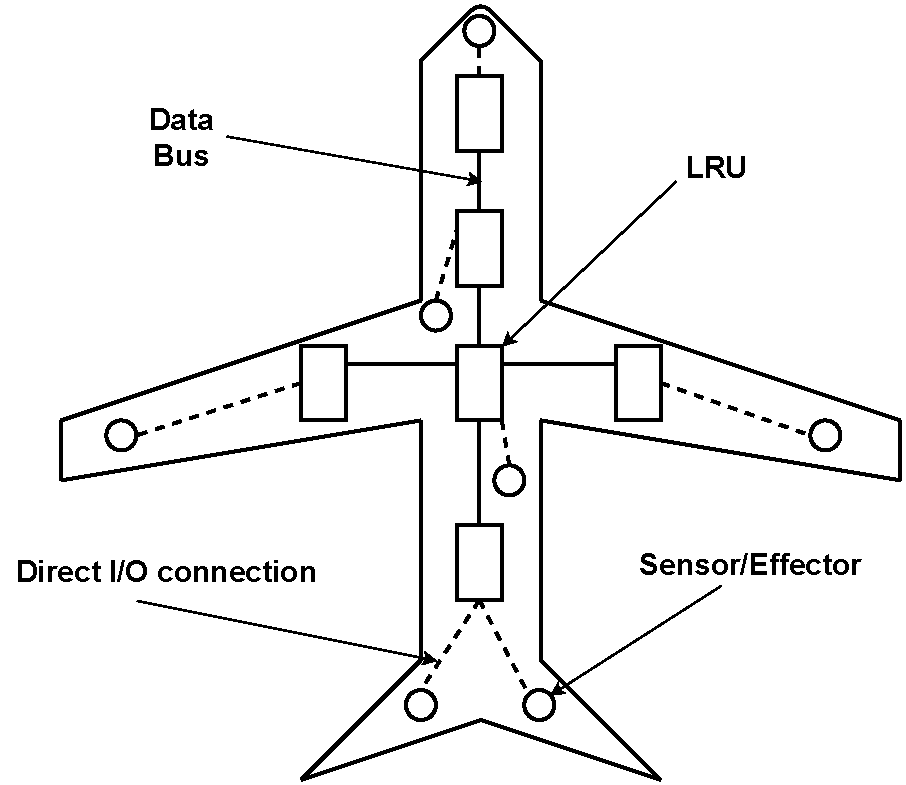
\includegraphics[width=1.0\textwidth]{figures/federated_architecture.pdf}
    \caption{Simplified visualization of the federated avionics architecture, showing \gls{lru}, sensors, effectors, and the global data bus}\label{fig:federated_architecture}
\end{figure}
\begin{figure}
    \centering
    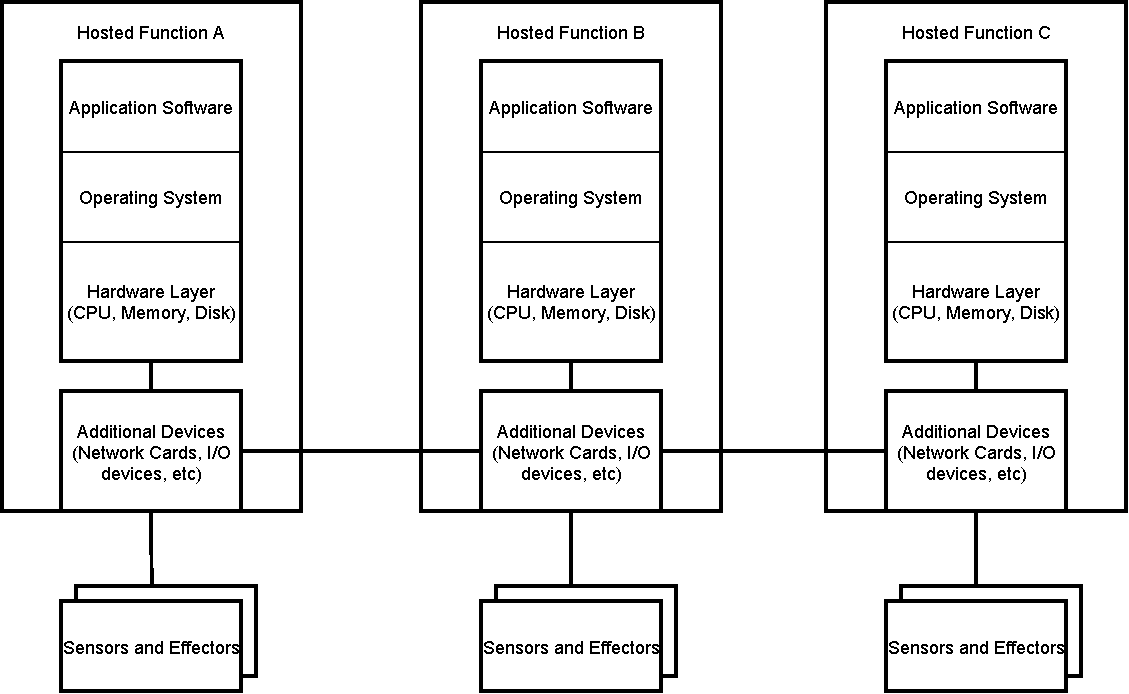
\includegraphics[width=1.0\textwidth]{figures/federated_architecture_components.pdf}
    \caption{Internal system architecture and interaction between \glspl{lru}}\label{fig:federated_architecture_components}
\end{figure}

\section{Integrated Modular Avionics}\label{section:integrated_modular_avionics}
\glsfirst{ima} is the direct successor of the federated avionics architecture. The idea behind \gls{ima}
is to consolidate the distributed hardware in one central flight cabinet. A Flight cabinet is very similar
to a rack in a datacenter. They can host multiple processing units, each comes with its own hardware stack
consisting of a \gls{cpu}, \gls{ram}, disk space and connectors for input and output\cite{prisaznuk1992integrated}. These servers are then plugged-in 
into the flight cabinet. Each server can host more than one avionic function and each function is allocated on partitions.
Partitions can be created on different ways and has been standardized in \gls{arinc653}\cite{vanderleest2010arinc}. The most common approach
is the use of a hypervisor (how this is implemented is being discussed in \autoref{section:workload_partitioning_strategies}). 
The flight cabinet provides power and required network connection to the plane's global data bus
as described in \gls{arinc629}\cite{isik2010arinc} or \gls{arinc429}\cite{fuchs2012evolution}. \gls{arinc629} is the successor of the data bus \gls{arinc429}.
Effectors and sensors communicate with the flight cabinet over \gls{arinc629}\cite{prisaznuk1992integrated}.
Sensors or effectors that are incompatible with \gls{arinc629} may communicate over remote data concentrators. Remote data concentrators are gathering data from sensors
or sending data to effectors over traditional \gls{io} connections. The gathered data or the received actions are communicated via \gls{arinc629} or \gls{arinc429}. Therefore,
remote data concentrators act as bridges between such devices and the data bus.
Using a central flight cabinet cannot replace all \glspl{lru} in the plane\cite{watkins2007transitioning}. These \glspl{lru} needs to be either integrated into the flight cabinet
or connected to the global data bus, for example via remote data concentrators. \autoref{fig:ima} depicts a simplified view on integrated modular avionics architecture in a plane.
The number of \glspl{lru} has been reduced and one central flight cabinet has been introduced. Remote data concentrators are working as bridges between sensors and effectors incompatible
with the data bus standard and the hosted functions in the flight cabinet. \autoref{fig:ima_components} shows the modules inside of such a flight cabinet. The flight cabinet
possesses multiple processing units. Each processing unit is comparable to a dedicated computer with its own hardware and operating system. These processing units
are being connected via a network layer and each processing unit hosts one or more hosted functions. Hosted functions are isolated from each other and have
a fixed predetermined set of resources and execution time.

\begin{figure}
    \centering
    \includegraphics[width=1.0\textwidth]{figures/ima.pdf}
    \caption{Simplified visualization of the integrated modular avionics architecture, showing sensors, effectors, cabinets and the data bus \glspl{lru}}\label{fig:ima}
\end{figure}

\begin{figure}
    \centering
    \includegraphics[width=1.0\textwidth]{figures/ima_components.pdf}
    \caption{View into a flight cabinet}\label{fig:ima_components}
\end{figure}

This system architecture has numerous advantages over the federated avionics architecture. Due to the more centralized approach \gls{ima}
is able to reduce weight via better cable management and less distributed processing units. Computing resources can be used more efficiently
via hosting multiple avionics functions on one processing unit. This leads to a higher system saturation. A positive side effect is less
energy consumption and a smaller ecological footprint. The reduced weight creates more space for cargo, fuel or passengers. 
Hardware consolidation leads to a consolidation of development efforts, which achieves cost and time savings\cite{watkins2007transitioning}.
The common processor allows the developer to focus on the hosted avionic function, enabling a better development experience and less error-prone
flight software. Separating software and hardware is a benefit during the certification process, because the certifying authority can certify
software and hardware separately. This has just another huge impact on cost and time savings. Additionally, upgrading the hosted function
becomes a lot easier, because of the hardware and software separation and less expensive hardware, due to standardized and more common
processing units. Another important benefit can be achieved via adopting the idea of open software and hardware. An open system architecture
with open standards can lead to a more competitive market due to industry-wide participation and exchangeability between hardware or
software applications. This way development and hardware costs can be reduced, because development cost gets distributed among all contributing
companies and mass production of standardized and open hardware shrinks marginal costs\cite{black2006open}. Moreover, the decoupling between hardware and software
can have a positive effect on new emerging companies, considering the lower costs\cite{watkins2007transitioning}. Software virtualization makes it easier to develop the
software, without buying expensive physical development kits. The software is being virtualized, tested and can be much later evaluated on real hardware, speeding up
the development process and time to market.

\section{Distributed Integrated Modular Avionics}\label{section:distributed_integrated_modular_avionics}
While \gls{ima} introduced a central architecture via consolidating computing resources into one central flight cabinet
\gls{dima} takes a different approach. \gls{ima} has shown that it is able to successfully reduce the number of components
in the plane with increasing number of hosted functions, because of its shared hosting infrastructure\cite{fuchsen2009preparing}.
Although this had positive effects on weight and cost management, there is room to improve in form of cable management.
Due to the centralized architecture it is necessary to connect every sensor and effector in the plane with the central flight cabinet
in the fuselage\cite{mccabe2009avionics}. This possible increase of cable length can be prevented via using ideas from the federated avionics and \gls{ima}.
\gls{dima} suggests a distribution of processing units, while taking into account the advantages of a central flight cabinet.
Instead of one central flight cabinet it is possible to redistribute the avionics functions over multiple flight cabinets distributed
in the plane's fuselage (see also \autoref{fig:dima}). This way it is possible to successfully exploit the advantages of the integrated architecture, while achieving
further improvements in the cable management\cite{li2012avionics}. Cable management is not the only possible adjustment for improvement.
The commercial cloud computing industry experienced a huge success over the last couple of years and these achievements can be used
for creating synergies between these two areas and applying cloud computing ideas in \gls{dima}. According to the \gls{nist} cloud computing is defined as:
\begin{displayquote}
\enquote{Cloud computing is a model for enabling ubiquitous, convenient, on-demand network access to a shared
pool of configurable computing resources (e.g., networks, servers, storage, applications, and services) that
can be rapidly provisioned and released with minimal management effort or service provider interaction.}\cite{mell2011sp}
\end{displayquote}
Although not all aspects of cloud computing are applicable on aviation, some of these aspects are.
One of these aspects is the separation into different service layers:
\begin{itemize}
    \item \gls{saas}
    \item \gls{paas}
    \item \gls{iaas}
\end{itemize}
\gls{saas} is handling all applications. \gls{paas} is responsible for the platform, where these applications
are running on (for example a hypervisor or services like webserver or databases). \gls{iaas} is the underlying
infrastructure (server, storages, networking). These three layers can be mirrored on the aviation world as follows:
\begin{itemize}
    \item \gls{saas}: Hosted functions
    \item \gls{paas}: The virtualized processing units or separation kernels
    \item \gls{iaas}: flight cabinets, remote data concentrators, the plane's data bus
\end{itemize}
Via separating each of these layers the aviation industry gains stronger standardization, more reliability and more effective
development workflows. Instead of selling one big monolithic system, separating makes it possible to develop products
for specific layers and interconnect them with the other layer via standards. These standards can be, as shown in \autoref{section:integrated_modular_avionics},
drivers for competition and exchangeability. Another aspect of cloud computing is the free and configurable allocation of applications\cite{li2012avionics}.
Dedicated storage, processor or sensor clusters would allow on-demand access from applications. Nevertheless it is a challenge to make this access reliable
and safe. Furthermore using standardized software may allow
interconnection between the plane and ground units (for example: real-time weather data transmitted from the ground to the plane).
This is partly comparable to the tactical data link of military units that get real-time radar data on their \gls{hsd}.

\begin{figure}
    \centering
    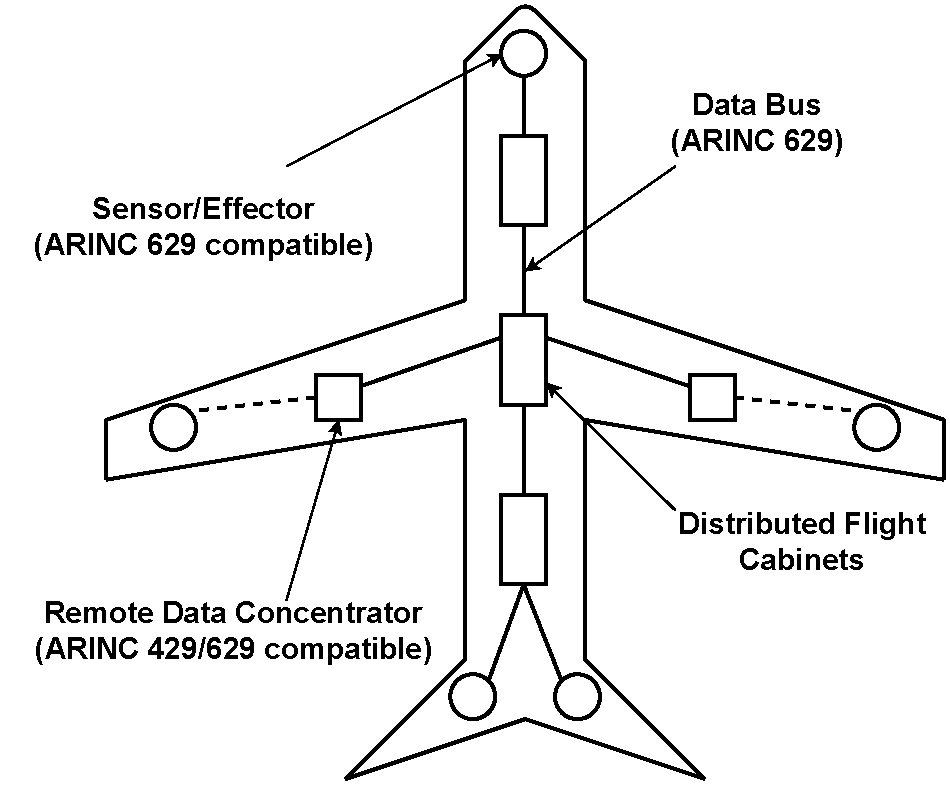
\includegraphics[width=1.0\textwidth]{figures/dima.pdf}
    \caption{Visualization of distributed flight cabinets}\label{fig:dima}
\end{figure}

\section{Workload Partitioning Strategies}\label{section:workload_partitioning_strategies}
Planes are composed of complex distributed systems with different tasks, requirements and environmental influences.
Every system has its own set of risks and possible impacts.
These different risks are known as \gls{dal} or \gls{idal} and have been defined
in the \gls{arp4754} as follows\cite{arp4754a2010guidelines}:
\begin{description}
    \item[A] Catastrophic system failures
    \item[B] Hazardous system failures
    \item[C] Major system failures
    \item[D] Minor system failures
    \item[E] No safety effect    
\end{description}

Due to these different risk levels it becomes important to isolate systems from each other. A system
with a low risk level should never have direct nor indirect impact on another system. In conclusion
the following measures are necessary to satisfy the safety and security requirements in planes:

\begin{itemize}
    \item Reserved \gls{cpu} time
    \item Reserved memory
    \item Reserved disk space
    \item \gls{qos}
    \item Network isolation
    \item Process isolation
    \item Privilege dropping
\end{itemize}

Reserved \gls{cpu} time means that every task has a strict time partition to work with.
Normally, cpu time is being shared on single processor systems. The operating systems simulates
parallelism via fast context switches. Multiple tasks are being executed consecutively switching
between them. This creates the impression that the system behaves parallel, but in reality it does not.
On multi processor systems real parallelism is possible. Reserved memory refers to a fixed memory
partition in the \gls{ram}. Reserved disk space refers to guaranteed space on a hard disk for storing
persistent data. Network isolation and Process isolatio ensures a noisefree and secure runtime environment.
Processes should not be disturbed by other processes either on process or network level. Furthermore,
each process has to drop privileges. Dropping privileges increases the safety and security of a service,
because it is less likely to interfere with other processes if the process has no privileges to do so.
\gls{qos} gives certain processes wit higher importance or risk level a higher priority. For example,
a system that controls the radar should have a higher priority than a system that just controls
the ambient lights in the passenger cabin.
Many of the above mentioned measures reveal other measures as direct dependencies. For example,
it is not possible to do proper \gls{qos} without an observable system that gets properly monitored.
Another example is the importance of security. On the first view security might be untangled of safety,
but in reality safety and security have a direct effect on each other. If the system is insecure it cannot
be safe and reliable, because every possible security incident could undermine all reliability promises.
The same applies to safety. An unsafe and unstable system cannot be considered secure, because these
weak points in the reliability might weaken the security. Just imagine a system that controls
permissions or security related functions. The system itself may be secure, but if it is unreliable 
it may has a direct effect on the security of other systems that depend on this particular system.
Additionally, planes have further constraints and requirements on software. One of these requirements
is a guarantee on response. Certain software systems in planes must respond before a given deadline.
This is called real-time communication. Real-time communication breaks down into the following types\cite{worn2006echtzeitsysteme}:

\begin{description}
    \item[Hard] The system has to satisfy all constraints. Responses are always on time. If a response would come too late it would inflict damage.
    \item[Firm] Executed tasks are worthless when their response does not satisfy the time constraint. No damage happens.
    \item[Soft] There are time constraints for requests and responses, but a tolerance exist. Delays are acceptable (as long as they fit in a specific time frame).
\end{description}

With all of these requirements it is obvious that there need to be technical implementations to satisfy all constraints.
The real-time constraints can be satisified via implementing real-time capabilities on operating system or kernel level.
Prominent examples are VxWorks' real-time operating system\cite{vxworks}, FreeRTOS\cite{freertos} or the real-time patches for the linux kernel\cite{realtimelinux}.
All other requirements are being solved either via virtualization or via containerization. There are two types of virtualization: Full virtualization and paravirtualization.
While full virtualization creates an almost full virtualized hardware including virtualized memory or \gls{io} devices, the paravirtualization does only virtualize
the software layer. The hardware stack will not be virtualized. Although this approach increases performance it is considered as less secure. With virtualization
it is possible to successfully isolate processes from each other and provide a dedicated workload partition for a specific software with its own \gls{ram} and \gls{cpu}.
The key element in this approach is the hypervisor. The hypervisor is the abstraction layer between the hardware, the software and their virtualized counterpart. 
Type 1 hypervisors run directly on the hardware, while type 2 hypervisors are running
on a dedicated host OS. Both hypervisors can usually virtualize a finite number of guests (finite, because the hardware resources are finite). Guests can be either applications or whole operating systems.
Many hardware provide direct support for virtualization, such as special instruction sets for \glspl{cpu}.
The containerization uses operating system or kernel level features to isolate processes or resources. In the Linux kernel this usually works via
making use of namespaces, kernel capabilities, control groups and union file systems. Linux namespaces have been heavily influenced by namespaces in Plan 9 (an alternative
operating system by Bell Labs) and zones in Solaris. Contrary to traditional virtualization, namespaces do not need a hypervisor layer, instead the kernel offers
a single system call called \emph{setns()}\cite{mannamespaces}. The Linux namespace \gls{api} consists of six dedicated namespaces, each responsible for a different isolation environment\cite{namespacelist}:
\begin{description}
    \item[mnt] responsible for filesystem mount points
    \item[pid] responsible for processes
    \item[net] responsible for the network stack
    \item[ipc] responsible for \gls{ipc}
    \item[uts] responsible for \gls{uts}
    \item[user] responsible for \glspl{uid}
    \item[cgroup] responsible for \glspl{cgroup}
    \item[time] responsible for time  
\end{description}
The first namespace \emph{mnt} specifies the filesystem hierarchy for the isolated process or a group of processes. With this namespace it is possible
to mount only a specific directory structure into the isolated environment. This ensures that a process from environment \emph{A} cannot
access files on the host system or in another environment. The \emph{mnt} namespace has become especially useful in combination with union file systems.
Union file systems are layered filesystems and allow to mount multiple directory structures over each other. Docker uses this technology for combining
different layers to a full docker container image. The second namespace \emph{pid} gives the system the opportunity to run multiple processes 
with the same \glspl{pid} on the host system. Running multiple processes with the same \gls{pid} on one system fulfills different purposes.
On one hand this provides reliability across different hosts. Via this approach it is possible to run a process with the same \gls{pid} in different
environments on different physical hosts. On the other hand it provides isolation. The process can only see other processes contained in the same namespace\cite{lwnnamespace}.
The \emph{net} namespace is responsible for everything network related. It provides the isolated environment with \gls{ip} addresses, ports, routing tables
and virtual network devices. \emph{net} is mostly being used for isolating network connections from each other. For example a namespace \emph{A} could provide
its own ports and internal IP addresses, while a namespace \emph{B} could provide the same port. The ports can be forwarded to the host via port-forwarding.
The \emph{ipc} namespace handles everything \glsfirst{ipc} related (message queues, Linux signals like \emph{sigkill} for killing processes etc).
For dealing with different hostnames in different namespaces the \emph{uts} namespace is being used. The last three namespaces implemented by Linux
are the \emph{user}, \emph{cgroup} and \emph{time} namespaces. \emph{user} is responsible for \glsfirstplural{uid} and \glsfirstplural{gid}. With
the namespace \emph{user} it is possible to different users or groups with the same \glsplural{uid} or \glsplural{gid} in different environment.
For example, having the \emph{root} user (the administrator account on Linux systems) in different isolated environments. The user \emph{root}
is identified by the \gls{uid} 0 and the \gls{gid} 0. Different times in isolated environments are provided by the \emph{time} namespace.
The last namespace, the \emph{cgroup} namespace, is responsible for the \glsfirstplural{cgroup}. A \gls{cgroup} enables the system to limit
and monitor resources inside of a namespace via providing a pseudo-filesystem called cgroupfs\cite{mancgroups}. Each \gls{cgroup} consists
of one or more processes and each process is being modified by a subsystem (also known as resource controller). Subsystems work as modifiers
for these processes. Via these modifiers it is possible to set specific limits or monitor the processes. For example, limiting the available
\gls{cpu} time or memory for a process, increasing the priority for network traffic, limiting access to \gls{io} devices or
monitoring events created by a process\cite{mancgroups}.

\section{Challenges}\label{section:Challenges}
% Here I want to list all challenges for my thesis
\nocite{*}
\printbibliography{}
\lstlistoflistings{}
\listoftables{}
\listoffigures
\glsaddallunused
\printglossary{}
\end{document}
